\part{Evaluation}
	\chapter{Introduction}
	The Evaluation chapter aims to take a critical look at the product and how well it satisfied the requirements. This will involve reviewing all hardware and software aspects of the system and discussing their strengths and weaknesses, with appropriate evidence to back up these discussions. 
	
	Following this will be an evaluation of the process that was undertaken to create the product. This will entail a discussion of any positives such as skills acquired and lessons learned as well as negatives such as performance problems. There will also be a discussion of potential alternative project plans using the benefit of hindsight to determine what might be done differently a second time around for the project to have enjoyed more success.
	
	Finally there will be conclusions and recommendations. Project aims will be compared against work carried out, and conclusions will be drawn summing up what has been carried out and what it means. Following this, recommendations for further work will be discussed in the context of the project's wider scope.
	
	\chapter{Product Evaluation}
	it's terrible 
	D:
	
	The Evaluation chapter aims to determine the strengths and weaknesses of the project. The choice of equipment and techniques will be evaluated, taking into account their original reasons for being employed and how useful they were during the project's development. In addition the strengths and weaknesses of the project's approach will be evaluated. Situations where the project's approach allowed for progress to be made or obstacles overcome will be described, as well as incidents where something different may have yielded more success. Finally the product itself will be evaluated. The original project requirements outlined in the analysis will be touched on again, and then the matter of whether or not they have been satisfied will be discussed. Attention will be given to aspects such as the original reasoning behind the objectives, the preliminary research (or possibly lack thereof) that contributes to the objectives success/failure as well as any strengths or faults during the project's synthesis. Finally, some conclusions on the project will be reached followed by recommendations for further work in the same vein. 
	
	\chapter{Product Evaluation}
	
	
	
	
	\chapter{Process Evaluation}
	\label{evaluation:processevaluation}
	%fitness for purpose and build quality sections from tor
	
	%talk about obvious issues with attempting to implement the SDK - get the actual linux error message(s)?
	%gives examples of previously attempted solutions and code snippets, e.g
	%i tried implementing manual getc and putc *actual code*
	%i tried using a byte lookup table on this *actual code*
	%i tried implementing a non-blocking interrupt handler attached to the rx channel *actual code*
	The way in which the project was approached had some strengths. The preliminary research into the relevant project fields helped in understanding what it was that precisely needed to be done to achieve the project goals. As well, I felt the review of tools and techniques was for the most part very helpful. The Terms of Reference featured some objectives that weren't entirely clear due to a few unknowns, most notably the objective dealing with how viable the drone was for SLAM and what the best way of storing map data would be. The tools and techniques review allowed for the specifics behind what to do here to be understood, as the preliminary investigation into file write speeds and how a radio transmitter would be integrated into the project helped me reach a decision on what to do.
	
	The project's process was not without its faults however. One of the biggest issues in the project's process was a grossly inefficient usage of time. The obstacle of establishing communication between the LIDAR sensor and the microcontroller came up right near the start of the project, but it was a great length of time before any actual success in having the two devices interface with eachother was realized. The significant amount of time trying to get this aspect of the project to work hurt the entire developmental process, and meant that even if everything else went perfectly there was still a lack of time. The problems compounded and caused a great deal of stress, which in turn made work on the project even worse. There are two key ways that this could have been avoided, or at the very least lessened in severity. The first is simply more research prior to the beginning of the project's development. Had more time been spent looking into the LIDAR, perhaps the modified SDK would have been stumbled upon sooner and this entire process could have been avoided. The second solution lies in the somewhat flawed project methodology. I still firmly stand by the prototyping methodology as being suitable for the product's development, but a more pronounced element of agility would have been good. The way prototyping was followed was having parts of functionality slowly iterated towards, but these iterations within themselves could have been approached in an agile fashion. This would have allowed for the prototyping to continue as intended, but would have additionally meant that the objectives were planned out in a more flexible manner so that blockers could be dealt with easier.
	
		\section{Choice of Equipment and Techniques}
	
	
	\chapter{Conclusions and Recommendations}
	
	
	
	
	
	
	
	\chapter{Blockers}
	Any minor issues encountered during development have been touched on in the implementation. Larger problems were encountered however that caused a more significant hindrance to the product's development. Some of these issues even involved the whole developmental approach having to be reconsidered. This chapter aims to explore these issues in depth by detailing what happened and how, if at all, these issues were overcome.
	
	\section{LIDAR Communication}
	A problem encountered near the start of the project was getting the SDK to work with the LIDAR sensor. The SDK's documentation states that the rplidar.h file simply needs to be included to gain LIDAR functionality, but when this was done the program gave file dependency errors during compile attempts. The most prominent error was an import problem where files within the SDK were unable to import the file sys/ioctl.h. Looking into this, ioctl.h appeared to be a linux kernel header file. The first attempt to fix this was simply making sure these kernel files were working properly, so APT was used to install or update the linux kernel headers. Other packages such as build-essentials were also installed, but none of these things fixed the problem. One other potential problem was that maybe there was a program somewhere relying on 32bit libraries which the 64bit Ubuntu OS didn't have, so APT was used to install the i386 architecture as well as some relevant packages to allow for better 32bit support. This didn't fix anything either. In a last ditch effort some of the kernal header files were actually copied into the LIDAR SDK, but this just resulted in other dependency problems coming up.
	
	Rather than continuing to spend time attempting to get the SDK working, it was decided to simply use the actual protocol that the SDK implemented. The protocol works by recieving request packets made up of certain bytes. Depending on what the bytes are, the LIDAR interprets the packet as a different command. These packets were created in the robot's program as arrays of bytes, and the Serial puts() command was used to send them to the LIDAR. getc() was then used within a task's main loop to retrieve the outputted data and it was printed to a terminal window. Relevant code snippets can be seen below.
	\begin{lstlisting}
	Serial pc(USBTX, USBRX);
	Serial device(D1, D0, 115200);
	
	char startRequest[] = {0xA5, 0x20};
	device.puts(startRequest);
	
	while (true) {
	pc.printf(device.getc()); 
	}
	\end{lstlisting}
	This had mixed results. Bytes were being recieved to the LIDAR but they were incredibly inconsistent. There wasn't a steady stream or a regular pattern to what was being returned. As well, bytes would stop coming through if the program was recompiled and reflashed or if the board itself was reset with the reset button. In addition to that the other commands listed in the protocol were even less effective. A stop request can be sent to the LIDAR so that it stops outputting data, but when this was sent any subsequent start requests wouldn't work and the LIDAR would stay dormant. To get the LIDAR working again the program itself had to be reset. The protocol documentation did state that a small period of time should be allowed to elapse between two commands being sent to ensure the LIDAR could process them, but even 3 to 4 seconds worth of a delay didn't fix anything here. Some requests had even more confusing results. The get health request is something that the documentation says returned 3 bytes, but when an appropriate request variable was made and sent to the device over the serial connection it returned only two bytes. Incidentally even if the command did work part of the response is an integer that represents the error code, but nowhere in the documentation could an actual table explaining what error each code corresponded to be found. 
	
	After consultation with the project mentor and some further studying of the Serial class, the potential solution of ensuring that data was retrieved via an interrupt rather than a constant loop presented itself. Having getc() constantly called whenever the while loop ran might have been causing problems, but with an interrupt handler it would only trigger when there was actually something there. Mbed's own documentation describes the RawSerial as a more suitable alternative to Serial for this approach so the device variable was changed to be of a RawSerial type. The code changes can be seen below.
	
	\begin{lstlisting}
	RawSerial device(D1, D0, 115200);
	
	device.attach(&rxInterrupt, Serial::RxIrq);
	
	void Rx_interrupt() {
	pc.printf(device.getc());
	}
	\end{lstlisting}
	This meant that the code to retrieve information from the device only ran when a character went into the RX buffer and was actually ready to be recieved. The strange behaviour with the stop request and some of the other requests was still present, but this resulted in LIDAR data being continuously and consistently printed to the console. This meant that at the very least there was data that could be worked with for now. These numbers were written in a binary representation to the Micro-SD card so they could be processed by the GUI, but there were problems there as well.
	
	This binary data would have to be turned into actual angle and distance numbers however. Fig \ref{fig:protocolbreakdown} is from the LIDAR protocol documentation, giving a breakdown of what byte in a returned scan packet corresponds to what information.
	
	\begin{figure}[ht]
		\centering
		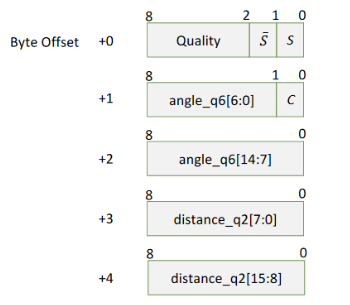
\includegraphics[width=.6\linewidth]{SYNTHESIS/protocolbreakdown.png}
		\caption{Protocol Breakdown}
		\label{fig:protocolbreakdown}
	\end{figure}
	
	So, for example, the first 6 bits of the first returned byte is used to store the scan's quality value. The idea behind the initial map processing software was to start at the beginning of the file containing binary scan data, then iterate through it by taking chunks of bits and storing them in variables.
	
	\begin{lstlisting}
	# Read in the bits according to the LIDAR response structure
	quality = f.read(6)
	inverseStart = f.read(1)
	start = f.read(1)
	angle_first = f.read(7)
	checkbit = f.read(1)
	angle_second = f.read(8)
	distance = f.read(16)
	\end{lstlisting}
	One small additional tweak that needed to be made was joining the first and second angle chunks together to form the full value.
	
	\begin{lstlisting}
	# Append the angle_q6 bits
	angle = (b"".join([angle_first, angle_second]))
	\end{lstlisting}
	
	The protocol documentation states that these aren't the true values however. The actual angle value is the binary value divided by 64 degrees, and the actual distance value is the binary value divided by 4 millimeters.
	
	\begin{lstlisting}
	# Turn binary into decimal
	# 'Actual heading = angle_q6/64.0 Degree'
	angle = (int(angle, 2) / 64.0)
	# 'Actual Distance = distance_q2/4.0 mm'
	distance = (int(distance, 2) / 4.0)/100
	\end{lstlisting}
	These points were then turned into mappable X and Y values. Despite all of this, none of this worked as intended. The produced maps made no logical sense, fig \ref{fig:failedmap} shows a map produced via this method from scans obtained from the inside of a rectangular box.
	\begin{figure}[ht]
		\centering
		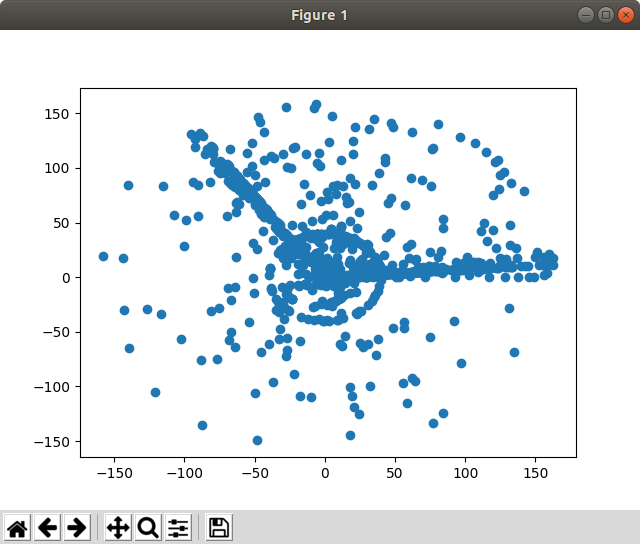
\includegraphics[width=.6\linewidth]{SYNTHESIS/failedmap.png}
		\caption{Resulting map of a box}
		\label{fig:failedmap}
	\end{figure}
	
	The generated values were printed, and it was observed that every now and then angles would be impossible values above 360. After all of this it was decided to go back to the drawing board and attempt to get the SDK working again since using the protocol was rapidly leading nowhere and burning time. Searching around on the mbed website stumbled across a robotic program that made use of a similar LIDAR system by SLAMTEC. The SDK in use there was a modified version that seemed to work fine with embedded systems, but still had all the necessary open licensing. This SDK was tested with the program and compiled fine, and is what was used to ultimately implement the robot's observational capability.
	
	\section{Memory Problems}
	It was previously assumed during the design and following some preliminary investigation into the available microcontrollers that the FRDM-K64F would be capable of storing the LIDAR readings in a temporary buffer before they are written to the file. To store the readings a two dimensional array was used, with each array entry containing a small array of two floats. To start off with the buffer used had a length of 16000, with each entry in itself containing an array of two floats (an angle and a distance). For the first few preliminary program tests this seemed to work fine, loops were used to write dummy entries to the array and the array was then written to a file to prove the process. During one test run however, a problem was shown in console along with a blinking red light on the mbed board indicating a runtime error.
	
	\begin{figure}[ht]
		\centering
		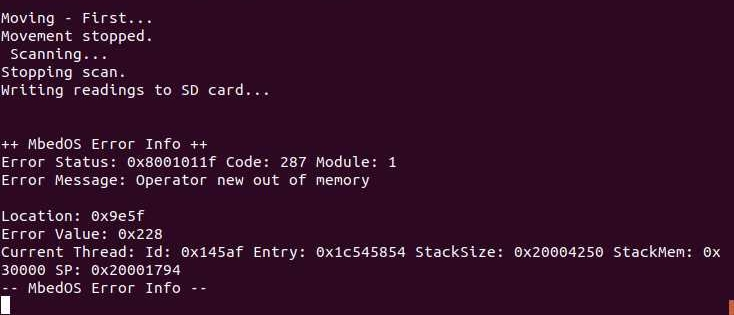
\includegraphics[width=.8\linewidth]{SYNTHESIS/memoryerror.jpg}
		\label{fig:memoryerror}
	\end{figure}
	
	This error began cropping up at the point where the program writes the buffer to a physical file. Despite it not being during the time when the readings buffer was actually filled out, the immediate reaction to the issue was simply to scale down the buffer. It made sense that perhaps too much space was being taken up by such a large variable, so it was halved to contain just 8000 angle distance pairs. The error was still encountered when compiling however, so just to see what would happen the array was decreased down to a significantly smaller size of just 1000. This issue still happened though, despite attempts to recompile and reflash the microcontroller as well as resetting the board with the reset button.
	
	\section{Scanning Inconsistency}
	One problem that repeatedly impeded development was the inconsistency in the LIDAR's scanning behaviour. Once development began to focus on writing real observational data into a buffer rather than filling it with dummy data just to prove the process, a number of issues began to crop up.
	
	The first was that occasionally entire batches of scan data would be zeroes. Every single angle and distance measurement would be a 0.0000000 float, with no changes to the buffer size making a difference. Pin connections were double checked and sometimes simply removed and plugged in again but then the scan straight after would result in the same thing happening. The troubleshooting section of the RPLIDAR A1M8 documentation was consulted. One suggestion was that the LIDAR core worked better once it had warmed up, and that it should be left spinning for a minute or so before it begins taking measurements. A simple task delay was introduced for 2 minutes before the main program loop began, but this issue would still come up sometimes. The quickest fix was generally to just recompile the program, and the issue would more often than not seemingly go away.